\documentclass[tikz]{standalone}
\usetikzlibrary{shapes,arrows.meta}
\begin{document}
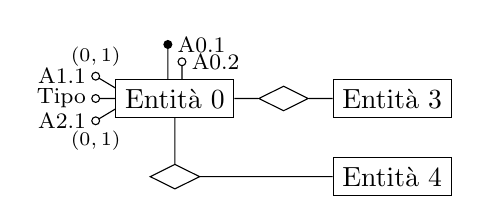
\begin{tikzpicture}
    \draw

    %%* Attributi:
    %%  node[draw, circle, inner sep=1pt,anchor=180, fill=black]{}node[right]{\footnotesize A}
    %%? Distanza orizzontale: E -(0.25,0.x)- A
    %%? Distanza verticale: E -(0,x * 0.22)- A

    %%* Cardinalità:
    %%  node[below right]{\scriptsize $(0,N)$}
    %%  node[above right]{\scriptsize $(0,N)$}
    %%  node[midway, above]{\scriptsize $(0,N)$}

    %%* Relazione:
    %%  node[draw, diamond, shape aspect=2, inner sep=3pt, anchor=90](r1){}
    %%  node[draw, diamond, shape aspect=2, inner sep=0.2pt, anchor=180](r2){R2}

    %%* Entità:
    %%  node[draw, rectangle, anchor=90](e1){}
    %%? Distanza verticale: E -(0.3)- R -(0.3) E
    %%? Distanza orizzontale: E -(0.75)- R -(0.75)- E

    (0,0)node[draw, rectangle, anchor=90](e0){Entità 0}
    (e0.110)--++(0,0.44)node[draw, circle, inner sep=1pt, fill=black]{}node[right]{\footnotesize A0.1}
    (e0.70)--++(0,0.22)node[draw, circle, inner sep=1pt, fill=white]{}node[right]{\footnotesize A0.2}

    (e0.170)--++(-0.25,.15)node[draw, circle, inner sep=1pt, fill=white]{}node[left]{\footnotesize A1.1}node[above]{\scriptsize $(0,1)$}
    (e0.180)--++(-0.25,0)  node[draw, circle, inner sep=1pt, fill=white]{}node[left]{\footnotesize Tipo}
    (e0.190)--++(-.25,-.15)node[draw, circle, inner sep=1pt, fill=white]{}node[left]{\footnotesize A2.1}node[below]{\scriptsize $(0,1)$}

    % [-{Stealth[round, length=5mm]}](0,-1.5)--(e0.270);
    % \draw
    % (0,-1.5)--++(-1.25,0)--++(0,-0.5)node[draw, rectangle, anchor=90](e1){Entità 1}
    % (0,-1.5)--++(1.25,0)--++(0,-0.5)node[draw, rectangle, anchor=90](e2){Entità 2}
    
    % (e1.270)--++(0,-0.22)node[draw, circle, inner sep=1pt, fill=white]{}node[below]{\footnotesize A1.1}
    % (e2.270)--++(0,-0.22)node[draw, circle, inner sep=1pt, fill=white]{}node[below]{\footnotesize A2.1}

    (e0.0)--++(0.3,0)node[draw, diamond, shape aspect=2, inner sep=3pt, anchor=180](r1){}
    (r1.0)--++(0.3,0)node[draw, rectangle, anchor=180](e3){Entità 3}

    (e3.270)++(0,-0.5)node[draw, rectangle, anchor=90](e4){Entità 4}
    (e0.270)|-(e4.180)node[fill=white, midway, draw, diamond, shape aspect=2, inner sep=3pt](r1){}
    ;
\end{tikzpicture}
\end{document}